\chapter{WSL2} \label{ChapWSL2}

In this section, we utilize the Windows Subsystem for Linux. This creates an
extremely lightweight virtual machine in within your Windows OS that emulates
the Linux kernel with a home drive.

%==============================================================================
\section{Installing WSL2}
%==============================================================================
Note, as of today (27th October 2021), the site \cite{microsoft2021wsl} states
that you can simply run
\begin{lstlisting}
    wsl --install
\end{lstlisting}
to install it. By default, it will:
\begin{itemize}
    \item Download the latest Linux kernel
    \item Set WSL 2 as your default
    \item Install the latest Ubuntu distribution.
\end{itemize}
You can, however, choose a different distribution to install by running
\begin{lstlisting}
    wsl --install -d <Distribution Name>
\end{lstlisting}
To see a list of distributions available for download and installation, run:
\begin{lstlisting}
    wsl --list --online
\end{lstlisting}
Below are the old instructions for installing WSL2.\\

To get i3 on Windows without a virtual machine (but technically a very
lightweight one is used), use WSL2. On the site \cite{microsoft2020wsl} , follow
the "Manual Installation Steps" for when you are not using the Windows Insiders
build.
\begin{enumerate}
    \item Open PowerShell as Administrator. If you use the Windows Terminal
        which can be obtained from the Microsoft Store, you can pin it to taskbar then
        press "shift+right-click" on the icon and click "Run as administrator".
    \item To enable the Windows Subsystem for Linux, in PowerShell, run
        \begin{lstlisting}
        dism.exe /online /enable-feature /featurename:Microsoft-Windows-Subsystem-Linux /all /norestart
        \end{lstlisting}
    \item Update your windows version if necessary
    \item To enable the Virtual Machine feature, in PowerShell, run
        \begin{lstlisting}
        dism.exe /online /enable-feature /featurename:VirtualMachinePlatform /all /norestart
        \end{lstlisting}
    \item Restart your machine
    \item To obtain WSL2, download the Linux kernel update package. The link for the download is
        available on step 4 of the website.
    \item Before installing a new Linux distribution, set WSL2 as the default version. To do this,
        in PowerShell, run
        \begin{lstlisting}
        wsl --set-default-version 2
        \end{lstlisting}
    \item Go to the Microsoft Store and install your favourite Linux distribution. If the "Install"
        button does not seem to work after you click "Get", you can go to your library and click
        "Install" there.
    \item Open Ubuntu and select your username and password. Username need not match your Windows
        OS user name
    \item To check that you have the correct version of WSL, in PowerShell run
        \begin{lstlisting}
        wsl -l -v
        \end{lstlisting}
    \item Run `sudo apt update', `sudo apt upgrade' and `sudo apt-get install
        build-essential' so that you have access to the standard operations.
\end{enumerate}
From here, your home directory can be found at "//wsl\$/Ubuntu/home/username"
(with backslashes instead of forward slashes as its a Windows directory address)

%------------------------------------------------------------------------------
\subsection{Errors}
%------------------------------------------------------------------------------
Here are some errors you might encounter and how to resolve them:
\begin{itemize}
    \item If you have an older machine, you may encounter
        "WslRegisterDistribution failed with error: 0x80370102 and error
        0x80070002" or other similar numbers. To remedy this, you may need to do
        two modifications to your BIOs. To access your BIOs modification menu,
        first restart your computer and continuously hit `F2' or some other
        button, depending on your CPU. When there, disable
        "Limit CPUID Maximum", then enable ``Virtualization Technology".
        Other names may be used for ``virtualization" such as ``SVM".
    \item For the error " WslRegisterDistribution  failed with error
        0xc03a001a", you may need to disable compression in a specific folder.
        Following runner-ed's answer in
        https://github.com/microsoft/WSL/issues/4299: Find the package under
        C:/Users/\tlangle your user name\trangle/AppData/Local/Packages and right click the
        folder, check advanced options and disable compression. Run the launch
        again.
\end{itemize}

%------------------------------------------------------------------------------
\subsection{Basic Operations and Config}
%------------------------------------------------------------------------------
Now to run Ubuntu in the Windows terminal. With your Windows Terminal pinned to
the start bar, simply right-click and select Ubuntu. To set Ubuntu as the
default, open Windows Terminal (can be opened to PowerShell or anything) and
press "ctrl+,". Then simply change "Default profile" to Ubuntu.\\

Now that you're operating in the Linux kernel, Vim should also be ready to go!
However note that, by default, you should be in your mounted Windows C drive.
Simply type `cd $\sim$' to change to the home directory. From here, you can git
clone your Linux .vim config and continue exactly as if you're on a Linux
machine!\\

To map the capslock key to escape, I recommend the following AutoHotKeys
command:
\begin{lstlisting}
    SetCapsLockState, alwaysoff
    Capslock::Esc
\end{lstlisting}

%==============================================================================
\section{VcXsrv}
%==============================================================================
Unix systems use the X Window System as their standard GUI environment.  Under
X, the "server" is the program that runs on your system to draw windows while a
"client' is a graphical program. The naming convention is a little confusing to
most computer users but, trust me, it makes sense.  While the Windows Subsystem
for Linux is a very well done method for running Linux software on a Windows
system, it lacks an X server so it is unable to run GUI applications by itself.
VcXsrv is an X server for Windows that's written to compile as a native Windows
application using Microsoft's Visual C++ (hence the name, Visual C++ X
Server).\\

The main motivation for using VcXsrv is so that we can utilize
Vimtex+Zathura+Synctex for forward and backwards searching while writing PDF
documents as discussed in Section \ref{SecFwdBckwdSynctex}. The initial idea to
incorporate VcXsrv for this was obtained from \cite{jong2020blazing}. However,
the installation process is quite involved and not fully captured in the
aforementioned medium post. We detail the installation process now.

%------------------------------------------------------------------------------
\subsection{Installation}
%------------------------------------------------------------------------------
\begin{enumerate}
    \item Go to the VcXsrv repo at \cite{articaproject2019vcxsrv} and follow the
        "Releases" link.
    \item Download the ``vcxsrv.1.17.0.0-3.x2go.arctica.installer.exe''
        whichever the latest release version is
    \item Run the installer
\end{enumerate}
Since WSL2 is a lightweight virtual machine, you'll need to do a couple of
things to ensure that your FireWall does not obstruct the connection.
\begin{enumerate}
    \item Following whme's TLDR answer from \cite{whme2020how}, in your .bashrc,
        add the following line:
        \begin{lstlisting}
            export DISPLAY=$(awk '/nameserver / {print $2; exit}' /etc/resolv.conf 2>/dev/null):0
            export LIBGL_ALWAYS_INDIRECT=1
        \end{lstlisting}
    \item Following whme's TLDR answer from \cite{whme2020how}, you need to
        disable Access Control on the Extra Settings. You can achieve this my
        first navigating to C:/Program Files (x86)/VcXsrv and opening
        "xlaunch.exe". This allows you to modify the settings. Navigate until
        you reach the "Extra Settings" page and check "Disable access control"
        as seen in the screenshot below:
        \begin{figure}[H]
            \centering
            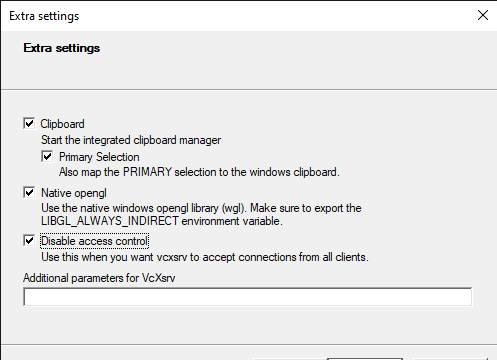
\includegraphics[scale=0.6]{vcxsrv_disable_access_control.png}
        \end{figure}
    \item Following \cite{alextsil2020steps}, go to Settings -\trangle Windows
        Defender Firewall -\trangle "Allow an app or feature through Windows
        Defender Firewall" and enable BOTH "VcXsrv windows xserver (X2Go/Arctica
        Builds) as seen in the screenshot below:
        \begin{figure}[H]
            \centering
            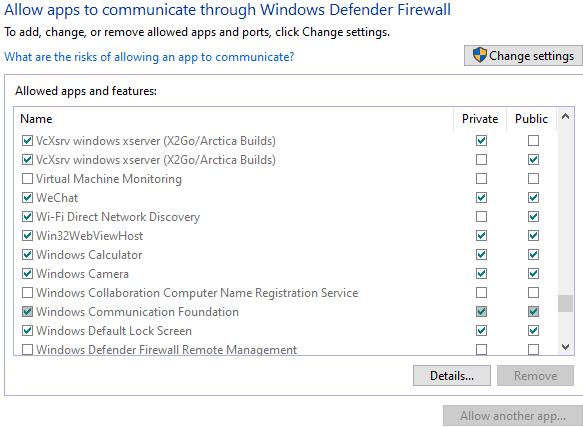
\includegraphics[scale=0.6]{vcxsrv_firewall.png}
        \end{figure}
    \item To test that VcXsrv now works, with Zathura installed, run "zathura
        name.pdf" and see if it opens.
\end{enumerate}
Note that the settings in Step 2 will revert itself. To accommodate for this,
you will be prompted in the next window to save the file "config.xlaunch". From
here, simply follow the instructions in Section \ref{SecAutostart} so that the
configuration is set after logging in.

%------------------------------------------------------------------------------
\subsection{Vimtex+Zathura+Synctex}
%------------------------------------------------------------------------------
Now you're almost ready to run Vimtex+Zathura+Synctex! You'll need to also
install xdotool by using "sudo apt-get install xdotool". To test whether this
works with VcXsrv following the suggestion in \cite{paulrougieux2020vimtex} from
lervag himself, run "xdotool search --class Zathura" and some numbers should
appear. From here, you should be good to go! Simply follow the steps laid out in
Section \ref{SecFwdBckwdSynctex}.\\

If this fails and you've given up on Zathura, you can alternatively use the
Sumatra PDF viewer. Once installed, simply add the following lines to your
vimrc:
\begin{lstlisting}
    let g:vimtex_view_general_viewer  = '/mnt/c/Users/Hwan/AppData/Local/SumatraPDF/SumatraPDF.exe'
    let g:vimtex_view_general_options = '-reuse-instance -forward-search @tex @line @pdf'
    let g:vimtex_view_general_options_latexmk = '-reuse-instance'
\end{lstlisting}
However, with this, you won't have access to forward and backward search via
synctex.

%==============================================================================
\section{Troubleshooting}
%==============================================================================

%------------------------------------------------------------------------------
\subsection{Vim Display Issues on Startup}
%------------------------------------------------------------------------------
When using Windows Terminal, you may notice that Vim has display issues when
starting up. Specifically, the columns might appear `diagonally' and only
resolves itself after playing around with the window i.e. toggling full screen
on and off. This is because the following settings in your vimrc:
\begin{lstlisting}
    set lines=62 columns=120
\end{lstlisting}
garbles the initial startup of Vim in Windows Terminal. Simply disable this
setting and the issue will disappear as suggested by waf's answer in
\cite{tompounceonGit2020vim}.

%------------------------------------------------------------------------------
\subsection{Visual Block Mode}
%------------------------------------------------------------------------------
To enter visual block mode in Vim, you need to press `ctrl+V'. However, in
Windows, this is bound to paste. Therefore, open the Windows Terminal settings
and open the `settings.json' file. Then locate the following code:
\begin{lstlisting}
        {
            "command": "paste",
            "keys": "ctrl+v"
        },
\end{lstlisting}
and change it to `ctrl+shift+v' if you like to mimic Linux.

%------------------------------------------------------------------------------
\subsection{Clash with Anaconda}
%------------------------------------------------------------------------------
You may notice that after installing Anaconda, when using
Vimtex+Zathura+Synctex, you may get the error `vimtex cannot find zathura
windows id' and forward/backwards search does not work. With some
experimentation, I discovered that in your .bashrc, the following block of code
that is added automatically with the installation of Anaconda:
\begin{lstlisting}
# >>> conda initialize >>>
# !! Contents within this block are managed by 'conda init' !!
__conda_setup="$('/home/hwangoh/anaconda3/bin/conda' 'shell.bash' 'hook' 2> /dev/null)"
if [ $? -eq 0 ]; then
    eval "$__conda_setup"
else
    if [ -f "/home/hwangoh/anaconda3/etc/profile.d/conda.sh" ]; then
        . "/home/hwangoh/anaconda3/etc/profile.d/conda.sh"
    else
        export PATH="/home/hwangoh/anaconda3/bin:$PATH"
    fi
fi
# unset __conda_setup
# <<< conda initialize <<<
\end{lstlisting}
causes the issue. Specifically, I noticed that if I comment out the line:
\begin{lstlisting}
__conda_setup="$('/home/hwangoh/anaconda3/bin/conda' 'shell.bash' 'hook' 2> /dev/null)"
\end{lstlisting}
then everything works fine with Vimtex+Zathura+Synctex. However, the terminal
command `conda' no longer works. When that line is removed, one no longer has
`(base)' at the beginning of each line in the terminal, so I suspect that there
is some clash with the anaconda environment. Therefore, a workaround follows
from \cite{drylabrebel2019how} where the answers suggest to run the
following command in terminal:
\begin{lstlisting}
conda config --set auto_activate_base false
\end{lstlisting}
which ensures that the Anaconda base envionment does not automatically appear by
default when the terminal is started.\\

This generally seems to fix the problem. However, I noticed that when compiling
tex documents using the LaTeX template used to write these notes, I get the
error `Compilation failed'. Despite this, you can still use `VimtexView' to open the
pdf and notice that compilation does work as the pdf does change. Additionally,
forward and backward search works as well. So I just ignore the error.
